\chapter{Origamist's algorithms \& data structures}
This chapter covers the most important computational algorithms, data structures and programming approaches the program uses.

\section{Representation of the origami model}
\subsection{Triangles and layers}
The model is stored simultaneously as a 3D model and 2D crease pattern. Both these models are represented by a set of triangles. Every 2D triangle corresponds to exactly one 3D triangle, and thus we will call the 2D triangle as the `origin' or `original' of the 3D triangle (because in the very first step, the corresponding 2D and 3D triangles are the same). The triangles are grouped to so called \emph{layers} of paper.
\begin{define}
A \emph{layer of paper} is a nonempty set of triangles meeting the following conditions:
\begin{itemize}
\item All triangles have their normals pointing in the same direction\footnote{This trivially holds for the original triangles}.
\item The original triangles form a single, nondegenerated and connected polygon\footnote{But possibly non-convex.} on the crease pattern.
\item The 3D triangles form a single, nondegenerated, connected and planar polygon.
\item Every triangle belongs to exactly one layer.
\end{itemize}
\end{define}

As a consequence of this definition, we see that the whole paper model can be parcelled into layers. A layer of paper can be imagined as the largest straight part of the paper bounded by creases or edges of the paper\footnote{But it is allowed for a layer to have its boundary at a crease of angle 0�. This means it doesn't always have to be the largest straight part, but it is guaranteed that a layer doesn't have its boundary somewhere `inside' (the boundary is always an edge of the paper or a crease).}.

What is the term of layer good for? A layer is always the smallest unit of paper that can be moved, bent, or rotated. If a fold would go through the interior of a layer, a crease is created in the layer and it is subdivided into more smaller layers\footnote{Convex layers always split to 2 parts, but nonconvex layers can generate more sublayers}.

\subsection{Fold lines}
Although it is not necessary to hold all the fold lines in memory\footnote{All fold lines could be just signalised by layers' boundaries.}, it shows that it is helpful to have a quick access to them. So, every triangle remembers all the fold lines it lies along, and all fold lines have links to the triangles lying along them. Moreover, the folds remember the direction of the fold (mountain/valley), so it can be used later in generating crease patterns or for displaying the just done operations (as described in \ref{sec:operationMarks}). They also remember their `age' in the number of steps they were last `touched' (used in a fold). The age can be used for blending old and probably unimportant creases.

\subsection{That's all we need}
The triangles, layers and fold lines are all we need to know to be able to correctly render and alter the model. More precisely, only 3D triangles and fold lines are needed, but layers and 2D triangles are needed for interaction with the model.

\section{How to represent the operations?}
\label{sec:operationsRepresentation}
Most operations consist of a set of lines, probably an angle or two, and\dots No, that isn't sufficient. Look at figure \ref{fig:chooseLayers}.

\begin{figure}
	\centering
	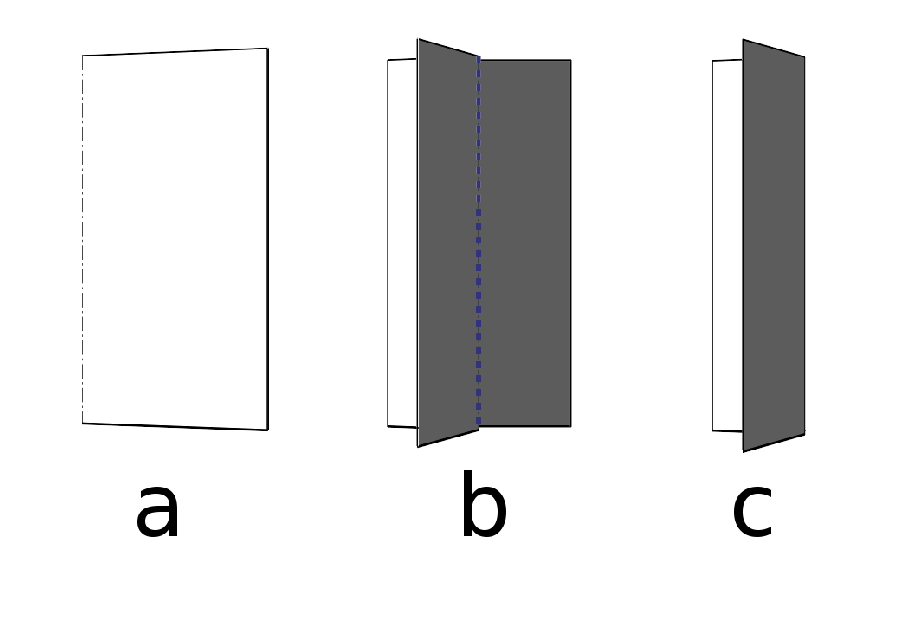
\includegraphics[width=150mm]{images/fold_layers}
	\label{fig:chooseLayers}
	\caption{Different layers that can be bent}
\end{figure}

The last thing to be specified is which layers of paper should be bent. As you can see in the figure, no layers are bent (a), the first layer is bent (b), or both layers are bent (c).

So we have it - lines, angles and layers. Lines and angles are easy to represent and address. Layers are worse. There is no unambiguous designation of the layers other than assigning them some artificial keys\footnote{We don't consider the option to label layers by themselves, because this is just useless - who would like to see the full list of triangles to be rotated in the diagram file? There must be a better option.}. But what keys? Should we index the layers according to the order they have emerged? That sounds really unnatural and like a bad design idea\footnote{What if the bending algorithm got changed and the order of layers' emerging with it?}.

I have finally found a naturally-looking set of keys. The mapping is based on the active line\footnote{It is never needed to select layers without the need to select a line altogether, so this makes sense.} (the line the currently created fold will be folded along). The line always lies in a layer. So take this layer and make a stripe perpendicular to it and having its border lines at the endpoints of the active line (it's actually always a segment). Then record all intersections of this stripe with another layers not parallel with the stripe\footnote{Bending a layer parallel with the stripe would mean bending a layer perpendicular to another layer we will bend, which makes no sense. Although such folds are possible, it would be better to divide them into two separate folds.}. Sort the intersections by the distance from the viewer\footnote{Since fold directions are dependent on the viewpoint, this brings no new dependencies to the algorithm.} (more precisely sort by the distance of their centres, because the intersections can have arbitrary angles towards the stripe and it wouldn't be clear what point to measure the distance from). Now, assign indices from 0 upwards to the sorted layers.

Although this key-mapping algorithm looks complex, it just does what people do naturally\footnote{How would I tell another person what layers to bend? I'd tell something like `Bend the first four layers,' or `Bend the topmost and bottommost layers.' Similar instructions can be found in many origami manuals. All these instructions refer to the same order of layers this algorithm defines.}.

So, in the data files, it is sufficient to first define the line to fold along, and then these keys can be used to describe the layers that will be bent. Figure \ref{fig:indexedLayers} illustrates this.

\begin{figure}
	\centering
	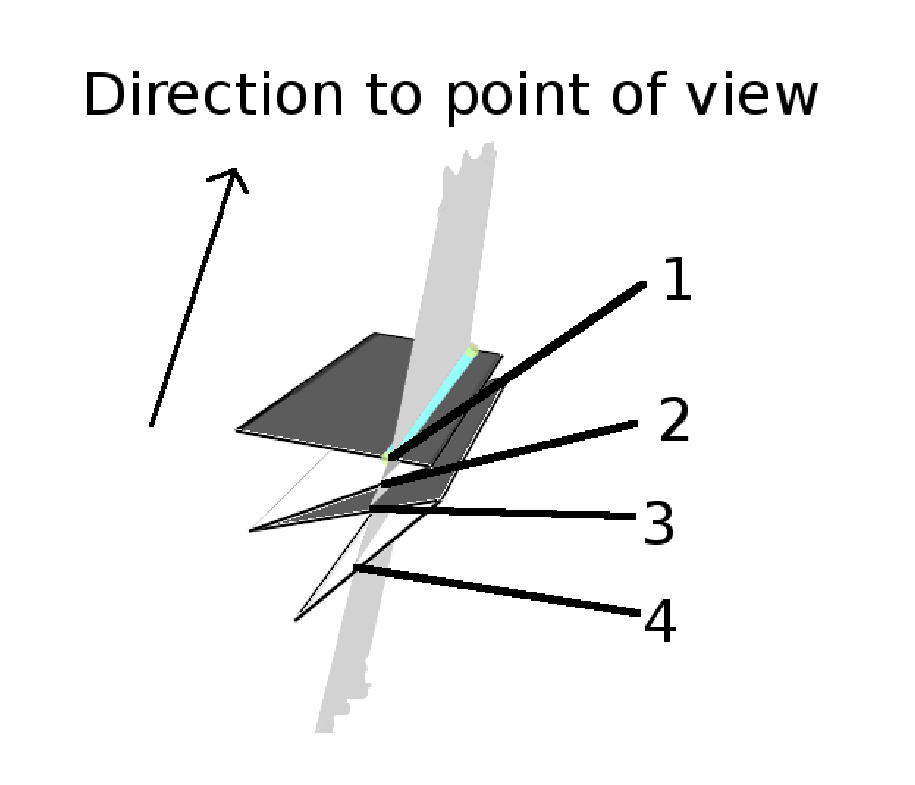
\includegraphics[width=150mm]{images/layers_indexing}
	\caption{The indices mapped to layers according to the active line (azure on the image).}
	\label{fig:indexedLayers}
\end{figure}

\section{How to bend the paper?}
\subsection{Which folds to implement?}
We will show that the ability to perform valley and mountain folds (let's call them basic folds) is sufficient for making any operation of those listed in \ref{sec:basicFolds}. 

It is possible that during the decomposed operation the paper will get into inconsistent state (eg. it can intersect and tear), but after completing the whole operation, it will be either consistent, or the operation was invalidly specified.

Thunderbolt fold is just a composition of two basic folds. Do the first one, then the second one, and that's it.

Inside/outside reverse folds can also be substituted with two basic folds (here the paper will be torn in between of the operations). It's worth noting that reverse folds don't need to specify angle of rotation, because there is only one nontrivial angle for which the operation will be valid (otherwise the paper would get curved). The angle is determined from the symmetry that reverse folds define. The symmetry is illustrated in figure \ref{fig:reverseSymmetry}

\begin{figure}
	\centering
	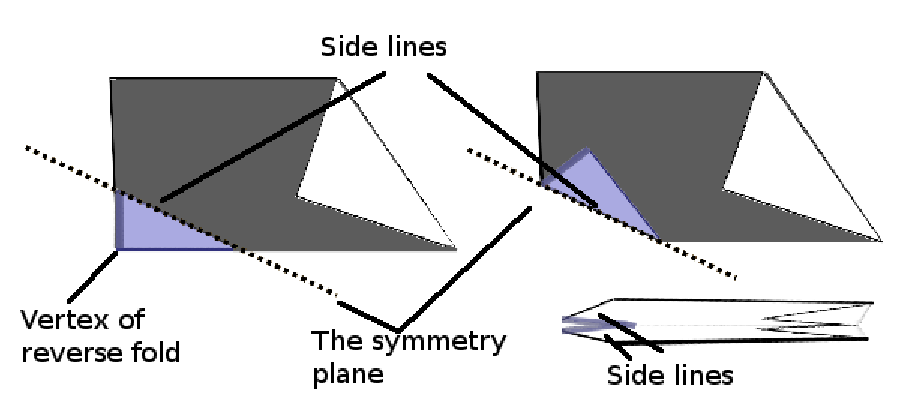
\includegraphics[width=150mm]{images/reverse_fold_symmetry}
	\caption{The symmetry of inside reverse fold.}
	\label{fig:reverseSymmetry}
\end{figure}

Inside/outside crimp folds are just double reverse folds and no additional paper tearing or intersecting can happen.

The pull operation also just rotates one part of the paper around the unfolded crease, so basic folds are sufficient.

The open operation is the most difficult, it could involve more layers to be rotated separately, but again, all of these steps will only be rotations of the paper around an axis (or multiple aces).

\subsection{The basic fold operation}
Let's get to the core of the folding. The operation is divided into two steps --- triangle subdivision plus fold line creation (let's call it `part 1'), and bending plus subdividing layers (calling it `part 2').

\subsubsection{Making creases}
Firstly, the layers involved in the triangle subdivision are determined by the algorithm from \ref{sec:operationsRepresentation}. All triangles having a fold line going through their interior are subdivided into two or three smaller triangles. All triangles carry the list of their neighbors, so these lists are updated. These triangles copy the appropriate fold line data of the old triangle and add the new fold line to their fold line data. Internally, the direction of the fold is taken relatively to the triangle's normal\footnote{Here it is important to mention that the triangle subdivision process must retain the same normal direction, which is no problem.}. So, this has been the first part of the process.

\subsubsection{Bending}
Then the bending comes to the scene. We need to detect all layers that will be rotated (that are not only those found in part 1, but also all layers `more distant' from the fold line but firmly connected to any rotated layer).

\subsubsection{Finding all layers to be rotated}
I use an eager algorithm for finding these layers. I begin with the layers from part 1. I subdivide them into more smaller layers and pick those that are to be rotated\footnote{This will be discussed later.}. Then I go to all neighbouring layers and check if they can be added to the to-be-rotated set. What are the terms for adding a layer's neighbour? Firstly, a newly added fold line mustn't lie between these two layers. If it did, one layer would surely have been in the part we want to rotate, whilst the other one would have been in the part we want not to rotate. And secondly (which is nearly implicit from what has been said former), the layer must be a neighbour of an already rotated layer. These two conditions are sufficient to find the right set of triangles to rotate. And then comes the easiest part - taking all the layers and rotating them around a single axis.

\subsection{Pitfalls}
There are still some unanswered questions on the folding algorithm. Let's take a look on them.

\subsubsection{What `half' to rotate?}
At the beginning of part 2, how do we choose the parts of the subdivided layers we want to rotate? Well, that's a question. We define a halfspace and take all layers the halfspace contains (the halfspace's border plane is the same as the plane of the stripe constructed for layer selection). What part of paper should `stay' and what should rotate? Geometrically, the results are the same. But the real 3D coordinates of the points will differ. One possibility is to let the user to select a point in the `half' of the model he wants to be rotated (these points are called `refPoints' in the application). Otherwise, we have to guess. Here is a little heuristic. Firstly, we just select any of the `halves' and find the layers to be rotated. But then the heuristic looks at the quotient of rotated and non-rotated triangles, and rotates the smaller of these two sets\footnote{This is based on the thought that the user mainly wants to rotate the smaller parts of paper, whilst the large remainder of the model should stay on place.}.

\subsubsection{Layers in composite operations}
The layer indexing and selecting algorithm fails while doing the second (third, fourth, \dots) basic operation during a composite one (eg. a thunderbolt fold). We could define the layers using this algorithm after doing each substep, the disadvantage is that the paper doesn't have to be in consistent state between the substeps. So another method for layer selection is applied to composite folds. The first substep has its layers of operation defined normally by the indices. After doing the first substep, it passes the rotated layers to the input of the second substep, and so on. This practice is based on the fact that all the composite operations work ordinarily with the same number of rotated layers for all substeps\footnote{And from a human point of view, these are `still the same layers'.}, so it perfectly matches the real folding process.

\subsubsection{Angle of rotation for reverse folds}
How to determine the angle of rotation for a reverse fold? We have already shown the reverse fold symmetry in figure \ref{fig:reverseSymmetry}. The symmetry is drawn as a line in the figure, but in fact it is a plane symmetry (the plane goes through the two side lines). So, to determine the angle, we just take the image of the reverse fold vertex (marked in the figure) and compute the angle between the image and the original.

\subsubsection{Multiple layers in the same plane}
Origamist could handle better the case when multiple layers of paper are folded so that they lie in the same plane. In this case, the ordering of layers for a fold operation isn't precisely defined. It doesn't do problems in the case of interactive model creation as long as the algorithm for layer indexing indexes the layers in the same plane equally. It will be needed to implement something like \cite{simulation} has --- the layers folded into a single plane remember their relative ordering, so it is possible to unambiguously identify them. This would also have better effect on the paper intersection check.

\section{Paper geometry checks}
Origamist implements two checks of the paper geometry. The paper tearing check, and paper intersection check.

\subsection{Paper tearing check}
This check is made very easily. Since all triangles know both their 2D (original) position and their 3D position, all that is needed to do is to iterate over 2D neighbors\footnote{Since the triangles carry the lists of their neighbors, this is really simple.} and check if they also are neighbors in 3D.

\subsection{Paper intersection test}This test is rather more demanding. To check if the paper doesn't intersect, we need to find all mutual intersections of layers and check if they are at most `touching'. Layers lying in the same plane are considered touching, layers with distinct parallel planes cannot intersect. The last possibility is that the layers' planes have a single common line. If the line isn't contained in any of the layers, the layers don't intersect. Finally, in the remaining case, we must check the touching. This is effectively done by constructing a halfspace with its border plane in one layer's plane, and checking if all of the other layer's points not lying in this border plane lie only on a single side of the defined halfspace (either all lie in the halfspace or none of them lies in it). Then the same is done with the halfspace's border plane being the second layer's plane.

This check runs asymptotically in $O(n^2)$, but practically it just consists from a small number of computations, and the count of layers isn't a very large number in basic and moderate origamis.

\subsection{When to run these checks?}
These checks cannot be run directly after a basic fold operation is done, because some composite operations need to get the paper into an invalid state during their operation. If we could do the check after the basic folds, it would simplify the checks, because it would be sufficient to take only the rotated layers into account. But since multiple basic folds can be done before the checks, we rather run the checks for the whole model\footnote{It could be sufficient to accumulate the rotated layers for all the substeps and do the checks for them.}.

\section{Delayed operations}
In Origamist editor, all operations are completely done as soon as they are defined. However, this is not suitable for the viewer and for manual generation. The classical origami manuals divide most operations into two steps. In the first one, only the creases the operation creates are marked. All the bending is done in the second step\footnote{This is for better clarity. It is simpler to show a fold's direction when it lies in a straight plane, than if it goes along an already bent crease.}.

The first idea I had was just not to perform the bending at all in the first step. But that would work only if just one simple operation is permitted per step (pureland origami). If multiple basic operations were done in a step and the bending weren't performed, the layer indexing algorithm could fail for the second and subsequent folds. Also, eg. the thunderbolt fold uses the list of layers rotated in the first substep to define the list of layers to be rotated in the second substep.

So, another approach is needed. Before the very first operation is done in a step, all triangles are instructed to save their current 3D position (every triangle has a special data field for this purpose). Then all bending operations are done normally, and after the last operation has been performed, triangles just restore their original positions --- but the created creases remain, which is exactly the desired result.

\section{Struggling with floating-point arithmetic}
The whole Origamist application is based on computing with floating-point numbers. Because a high precision is needed in the application, the Java type \emph{Double} is used. But even this isn't sufficient for the operations to be precise. I try to have all the model's vertices' coordinates between $-1$ and $1$, because Double has the highest density in this interval, so it is supposed to have the least rounding errors.

All comparisons are done by checking if the absolute value of the difference of the compared numbers is less than a specified $\epsilon$. What $\epsilon$ to take? I use $10^{-6}$ as it has a good mapping to the reality. As the longest side of the paper has the length of 1 unit (usually about 20 cm in physical world), the epsilon corresponds to $2*10^{-7}$ meters. Due to the thickness of a paper sheet (being something like $10^{-4}$ meters) this $\epsilon$ value seems to be appropriate.

This $\epsilon$ is thus good for operations on the paper's vertices. But what about comparing angles or other paper-unrelated numbers? Well, for simplicity, Origamist uses the same $\epsilon$ everywhere, but the precision of computations would be better if the $\epsilon$ were scaled according to the unit it is used for. \cite{dawson} provides some hints on how could this be done better.

\subsection{$\epsilon$-comparing maps?}I had the idea to develop a map (a tree) that could store 3D points or lines and search among them to return those that are $\epsilon$-equal to a given search key\footnote{In order to store the neigbors lists and such things outside the triangles.}. Classical approaches aren't successful. Hashmaps don't work because $\epsilon$-equal items don't have to have equal hash code, and there is no suitable mapping that could assign the hashcodes reasonably\footnote{Partitioning the space to $\epsilon$-equal blocks doesn't work, because if you put a number from the lower bound of one block into the map and then search for a number even smaller, the search will fail even if the distance if these items is less than $\epsilon$.}. Classical binary search trees also fail quickly with floating-point numbers.

I had the idea to use multidimensional interval trees, which could work for this purpose. Or R-trees could also work. But instead of implementing these complex data structures\footnote{Java doesn't provide a default implementation.}, I have found out that they aren't needed. All the information that seemed to need these maps could be stored somehow else. Eg. the list of triangles' neighbors is stored inside the triangles and so on. This finally seems to be the most effective approach.

\subsection{What about rational numbers?}The use of rational numbers for all computations would greatly increase the precision of the computations. But there are some facts that disallow this. The main problem are angles\footnote{Because Origamist doesn't need any other `irrationalizing' operations like $\log$ or square roots.}, which generally have irrational sines and cosines (and those are used in computing the rotations). So, if we restricted to angles with rational sines and cosines, it maybe would be possible to switch to rational numbers. But then we couldn't represent the often used angles like 45� (which has both sine and cosine equal to $\sqrt{2}/2$). So this question remains open.

\section{Operation marks}
How to place the marks for performed operations onto the model (in viewer and manuals)? There are no precise rules on how to do this, so I have chosen a heuristic which looks to produce good results.

For every fold operation the furthest rotated point can be determined (furthest from the rotation axis). Then this point's position determines one enpoint of the mark, and the nearest point on the rotation axis to this furthest rotated point determines the centre of the mark. So we have two points and can properly rotate and scale the mark.

For non-fold operations (like rotation), the marks are placed around the model's bounds.
